
Um motor DC é fundamentalmente uma máquina elétrica de corrente contínua, que
converte energia elétrica de corrente contínua em energia mecânica. Máquinas
elétricas de corrente contínua são mais fácies de controlar e oferecem uma
grande faixa de velocidades \cite{Maquinas_eletricas}. Devido a essas
características, tornam-se ótimas candidatas para uso em eletrônica e robótica,
pois podem ser usadas com baterias. Para controlar a velocidade de um motor,
é necessário o uso de um encoder, que converte o sinal de posição em um valor
mensurável de velocidade angular.


Para os fins deste trabalho, optou-se pelo uso de um motor DC de 6V 210rpm, 
com taxa de redução de 1:34. O encoder escolhido é um encoder magnético, já
vem acoplado ao motor empregado, com 11 PPR (\textit{Pulses Per Revolution}).



\begin{figure}[h]
	\centering
	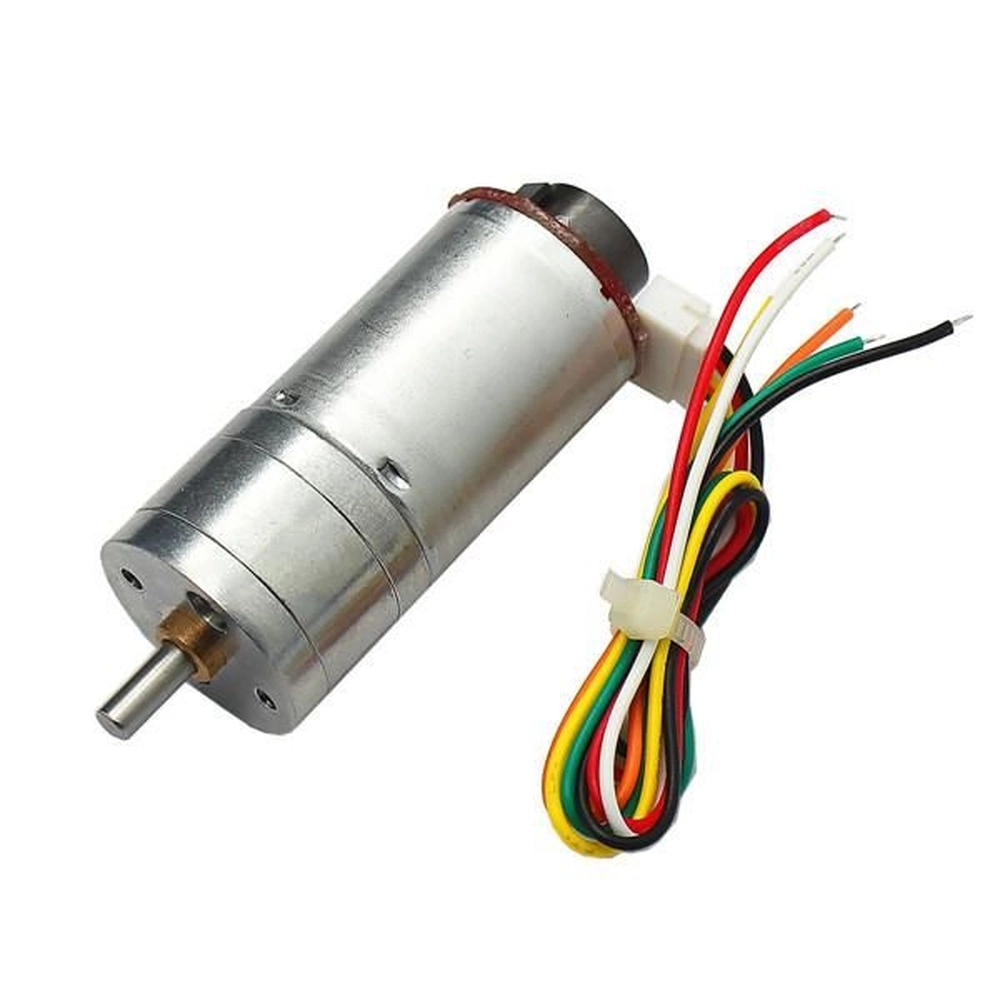
\includegraphics[width=0.7\textwidth]{figures/CHR_GM25_370}
	\caption{Motor DC 6V \cite{motor_dc_6v_encoder}}
\end{figure}

\begin{quadro}[htb]
	\caption{\label{Especificacoes_motordc_6v}Especificações do motor DC 6V}
	 \begin{tabular}{|c|c|c|c|}
		\hline
		\textbf{Componente} & \textbf{Quant} \\ \hline
		Tensão nominal & DC 6V  \\ \hline
		Velocidade sem carga  & 210RPM 0.13A  \\ \hline
		Eficiência máxima & 2,0kg.cm/170rpm/2,0W/0,60A   \\ \hline
		Poder maximo & 5,2kg.cm/110rpm/3,1W/1,10A   \\ \hline
		Torque de parada  & 10kg.cm 3.2A    \\ \hline
		Taxa de Redução do Retardador & 1:34  \\ \hline
		Resolução do salão & Razão Hall x 34,02 = 341,2PPR  \\ \hline
	\end{tabular}
	\fonte{\cite{chinhai_motor}}
	\end{quadro}
	
\subsection{Encoder magnético}

	Por se utilizar um encoder PRR, são produzidas duas ondas quadradas como saídas,
	A e B \cite{encoder_ppr}. As duas possuem 90° de fase entre si, e, caso a onda A
	esteja adiantada em relação a B (\ref{encoder_ppr_ab}), o sentido de rotação é
	positivo (anti-horário).

\begin{figure}[h]
	\centering
	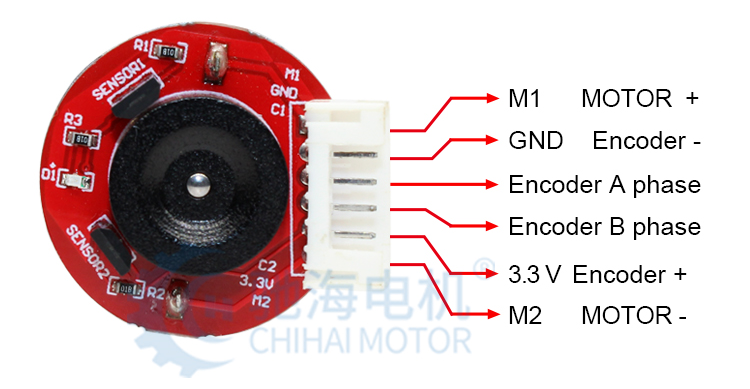
\includegraphics[width=0.6\textwidth]{figures/encoder_holzer}
	\caption{Encoder holzer \cite{motor_dc_6v_encoder}}
\end{figure}

\begin{figure}[h]
	\centering
	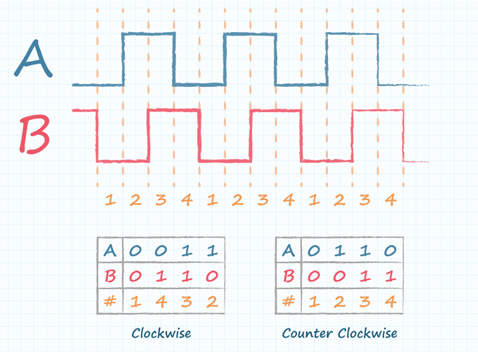
\includegraphics[width=0.7\textwidth]{figures/encoder_pulso_ab}
	\caption{Ondas quadradas resultantes dos pulsos de saída do encoder \cite{encoder_ppr}}
	\label{encoder_ppr_ab}
\end{figure}


\subsection{Driver para motor}

	Motores não podem ser ligados diretamente nos pinos de um microcontrolador, 
	é necesário um circuito que permita a baixa corrente do microcontrolador controlar correntes mais altas, como as de um motor DC.
	Drivers podem ser usados em uma variedade de tensões de entrada e permitem o controle da velocidade por PWM \cite{toshiba_ponte_h}.

	O driver a ser usado é do tipo ponte H. A Ponte H permite que a polaridade da alimentação do motor DC seja trocada.
	Devido a inercia do motor, ele continua girando mesmo quando a energia é retirada,  
	mas a ponte H pode curto-circuitar os terminais do motor, gerando uma força eletromotriz de frenagem.
	Outra razão para uso de um driver ponte H, é lidar com a tensão gerada pelo motor quando o rotor continua a girar depois de remover alimentação, 
	o motor se comporta com um gerador nesse momento, e a ponte H fornece um caminho livre para essa corrente gerada pelo rotor.


\begin{figure}[h]
	\centering
	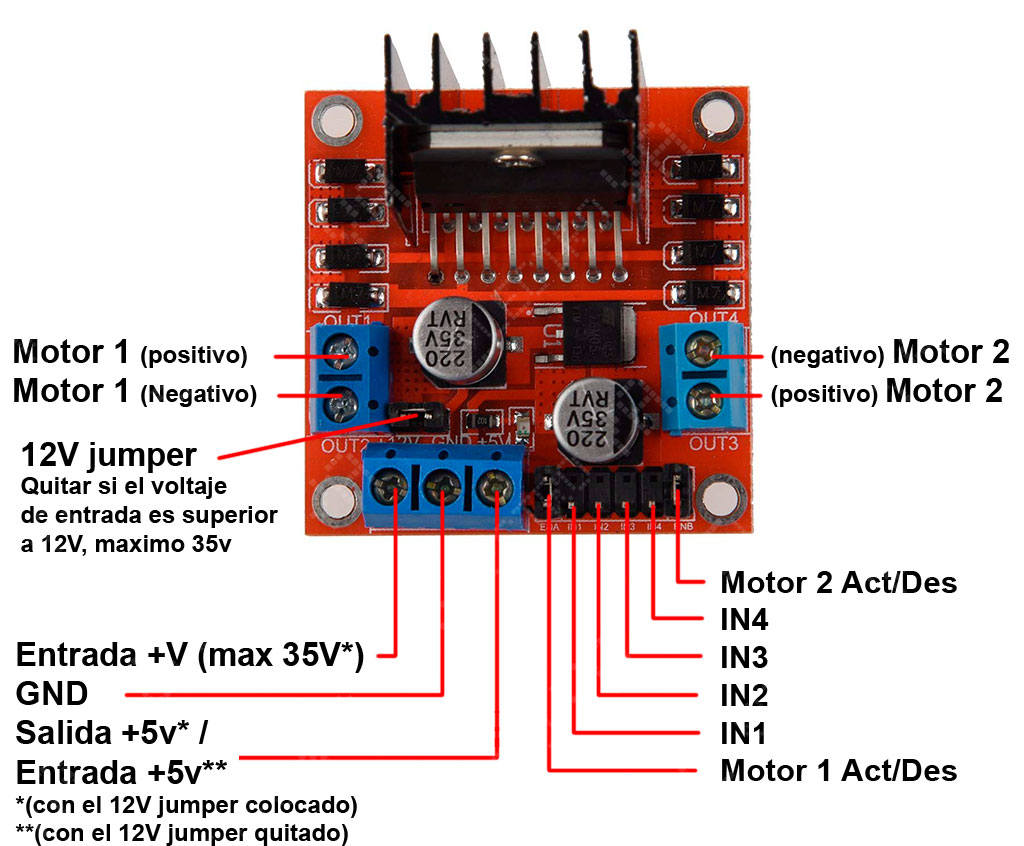
\includegraphics[width=0.7\textwidth]{figures/l289n}
	\caption{Driver Ponte H L289N \cite{l289n}}
\end{figure}
